
\documentclass[12pt,letterpaper]{hmcpset}
\usepackage[margin=1in]{geometry}
\usepackage{graphicx}
\usepackage{amssymb}
\usepackage{gensymb}
% info for header block in upper right hand corner
\name{Name: \underline{\hspace{3cm}}}
\class{Math 45, Section \underline{\hspace{1cm}}}
\assignment{HW 01}
\duedate{March 9th, 2018}

\begin{document}
\section*{}





%------------------------- Problem 1 -----------------------

\begin{problem}[Problem 1]
By differentiating each function verify that $y_i(t)= e^{-t}$ and $y_2(t) = \sinh t$ both satisfy the differential equation $y^{\prime\prime}-y= 0$ Is$ y(t) = Ay_1(t) +By_2(t)$ where $A$ and $B$ are arbitrary constants, also a solution? Why or why not?
\end{problem}
\newpage

%------------------------- Problem 2 -----------------------

\begin{problem}[2. ]
   Suppose that an object is moving in a straight line with constant acceleration $a \exists \mathbb{R}$ Use properties of integration to show that the position of the obeject as a function of time $t$ is given by; 
   $$ p(t) = \frac{1}{2}at^2+v_0t+p_0$$
   where $v_0$ and $p_0$ denote the velocity and postion at time $t=0$. Start by observing that accleeration is the second derivitave of position, thus; 
   $$ p^{\prime \prime} (t) = a$$
   Be careful in your solution to rigorously justify each step. 
\end{problem}

\begin{solution}
    \vfill
\end{solution}

\newpage

%------------------------- Problem 3 -----------------------

\begin{problem}[3]
   Verify that; 
   $$ y(t) = e^{t^2} \int_{0}^{t} e^{-s^2}ds+e^{t^2}$$
   is a solution to the differential equation $y^{\prime} -2ty = 1$, with the inital condition $y(0) = 1$
\end{problem}

\begin{solution}
    \vfill
\end{solution}

\newpage

%------------------------- Problem 4 -----------------------

\begin{problem}[4]
   Examine Student W's work on the following problem. What did the student do correctly? What mistake(s) did the student make? What is a more correct response to the problem, and what would you say to help the student understand how to correctly complete the problem? 
\end{problem}
   \begin{figure}[h]
   \centering 
   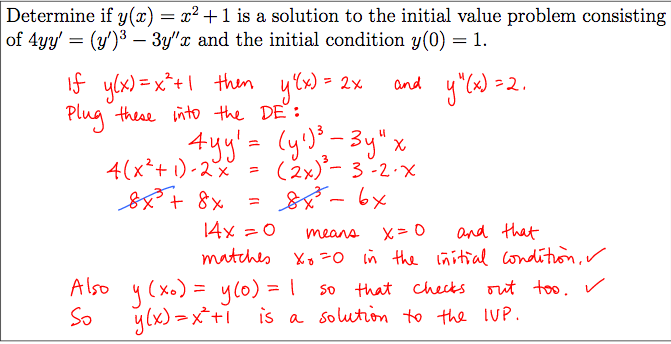
\includegraphics[width = 5in]{StudentW}
   \end{figure}
\begin{solution}
    \vfill
\end{solution}

\newpage


\end{document}
